\documentclass[10pt,journal]{IEEEtran}  %10pt, sans, memo

\usepackage{subcaption}
\usepackage{amsthm}

\usepackage[utf8]{inputenc}

\usepackage{tikz}
\usepackage{tikzscale}
\usepackage{pgfplots}

\usepackage{booktabs}
\usepackage{graphicx}
\usepackage{mathtools}
\usepackage{breqn}
\usepackage{natbib}

\usepackage{hyperref}

\bibliographystyle{ieeetr} 

\author{Jonathan Dyer}
\date{\today}
\title{High Resolution Space-based Remote Sensing Trade Space}
\hypersetup{
 pdfauthor={Jonathan Dyer},
 pdftitle={EO Modalities},
 pdfkeywords={},
 pdfsubject={},
 pdfcreator={}, 
 pdflang={English}}

\newcommand{\includepgf}[3]
{
  \begin{figure}[h!]
  \centering
  \includegraphics{#1}
  \caption[]{#3}
  \label{#2}
  \end{figure}
}
\DeclarePairedDelimiter{\abs}{\lvert}{\rvert}
\DeclarePairedDelimiter{\norm}{\lVert}{\rVert}

\begin{document}

\newtheorem{mydef}{Definition}

\makeatletter
\newcommand\footnoteref[1]{\protected@xdef\@thefnmark{\ref{#1}}\@footnotemark}
\makeatother

\author{Jonathan~Dyer,~\IEEEmembership{Member,~IEEE,}
        Dirk~Robinson,~\IEEEmembership{Member,~IEEE,}
        and~Paul~Boerner,~\IEEEmembership{Member,~IEEE}%
}

\markboth{Journal of \LaTeX\ Class Files,~Vol.~14, No.~8, August~2015}%
{}
        
        
\IEEEtitleabstractindextext{%
\begin{abstract}
The abstract goes here.
\end{abstract}


% Note that keywords are not normally used for peerreview papers.
\begin{IEEEkeywords}
IEEE, remote sensing, satellite, spacecraft, high resolution.
\end{IEEEkeywords}}


% make the title area
\maketitle

\IEEEdisplaynontitleabstractindextext

\section{Introduction}
\label{sec:introduction}

The trade space for high resolution remote sensing spacecraft is nuanced and many assumptions made historically in the architecture of such systems are less valid in light of rapid developments in image sensors, attitude control and other spacecraft subsystems.  In this article, we explore the trade space specifically in light of the recent trend toward smaller, lower cost spacecraft.

\section{Performance Trade Space}
\label{sec:trade_space}

The high resolution imaging trade space is fairly well constrained by a few driving requirements which are, in turn, driven by four primary mission needs:

\begin{enumerate}
\item Phenomenology
\item Image Quality
\item Collection Capacity
\item Cost
\end{enumerate}

\emph{Phenomenology} refers to the phenomenon being sensed or study and drives things like the spectral range, signal-to-noise ratio (SNR) and resolution required.  

\emph{Image Quality}, likewise, drives resolution and SNR.  

\emph{Collection capacity} drives many system variables both within the payload (such as swath width) as well as elsewhere in the spacecraft (collection rate, attitude control agility).  

\emph{Cost} is an increasingly important constraint placed on both technology selection and physical dimensions of the spacecraft.

We will spend significant time studying the system trades impacting Image Quality, Collection Capacity and Cost.  Phenomenology will only be addressed in passing.

\section{Remote Sensing Driving Requirements}
\label{sec:requirements}

Taken together these mission needs define the requirement trade space we will study here.

Table \ref{table:drivers} shows the effect of many mission-level needs on lower-level requirements.
\begin{table}[h!t]
\resizebox{.45\textwidth}{!}{%
\begin{tabular}{@{}ll@{}}
\toprule
\textbf{Requirement} & \textbf{Drives} \\ \toprule
Resolution & \begin{tabular}[c]{@{}l@{}}Aperture Diameter\\ Altitude\end{tabular} \\ \midrule
\begin{tabular}[c]{@{}l@{}}SNR \& Dynamic Range\end{tabular} & \begin{tabular}[c]{@{}l@{}}Stabilization\\ Detector Full-well\\Optical $F^\#$\end{tabular} \\ \midrule
Swath Width & \begin{tabular}[c]{@{}l@{}}Optical Complexity\\ Detector Width\\ Data Volume\end{tabular} \\ \midrule
Collection Rate & \begin{tabular}[c]{@{}l@{}}Stabilization\\ Detector line-rate\end{tabular} \\ \midrule
Spectral Sampling & \begin{tabular}[c]{@{}l@{}}In-track FOV\\ Camera filters\\ Semiconductor Bandgap\end{tabular} \\ \bottomrule
\end{tabular}%
}
\centering
\caption{System Performance Drivers}
\label{table:drivers}
\end{table}

It is important to note that many of these requirements are tightly coupled.  For example chosing a high resolution requirement directly impacts the difficulty of meeting other requirements:

\begin{itemize}
\item High resolution drives either a reduction in achievable SNR or a increase in required integration time and associated tighter ACS stability and more powerful image stabilization
\item Recovering SNR at high resolution drives detectors with high line-rate (for digital oversampling) and/or significant analogy stabilization (TDI or optical)
\item High resolution increases focal plane width and data intensity or reduces swath width while still increasing data intensity

\end{itemize}

In order to facilitate discussion of these system trades, we will define some key system performance metrics in the following sections but first we will introduce the non-dimensional parameter $Q$.

\subsection{$\frac{\lambda F^\#}{p}$ or Q}
\label{sec:q}

The system parameter $Q$ is defined as:

\begin{equation}
Q = \frac{\lambda F^\#}{p}
\label{eq:Q}
\end{equation}
and is essentially a measure pixel sampling in the spatial domain relative to the Nyquist criterion.  Nyquist says that to completely reconstruct a band-limited system, the spatial sampling frequency. 
$$\rho_s = 1/p \geq 2 BW_{opt}$$

Because we always sample to DC, the optical bandwidth $BW_{opt}$ is replaced by the diffraction cutoff frequency.
$$\rho_c = \frac{1}{\lambda F^\#}$$

Thus $Q$ is a measure of Nyquist sampling where $Q=2$ is critically sampled.  Most systems, however, operate at $Q < 2$ and hence incur some spatial aliasing.  There is little reason to operate at $Q > 2$ as the optics do not pass spatial frequency information there so the additional sampling is essentially wasted.

\begin{figure}[h!]
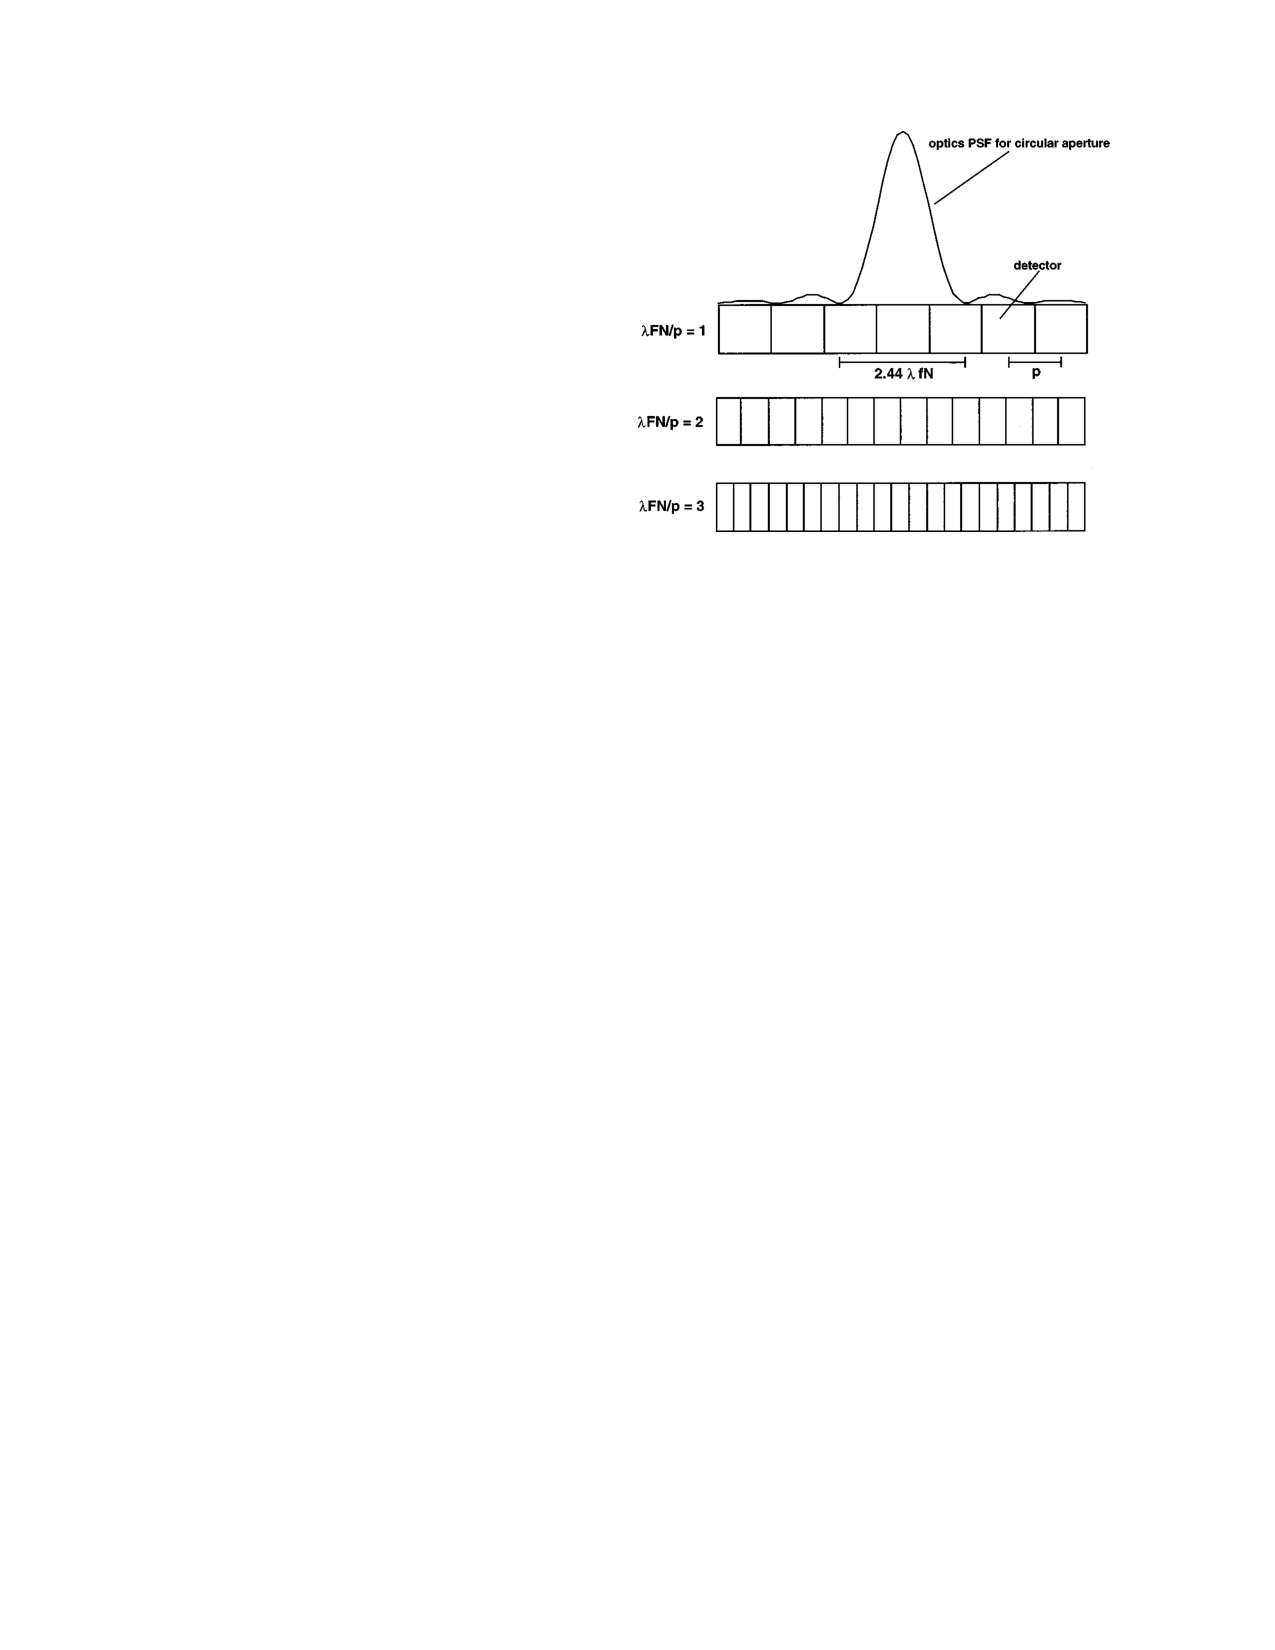
\includegraphics[width=0.42\textwidth]{figures/Q_fiete.pdf}
\caption{Spatial interpretation of Q sampling a diffraction-limited PSF.  Adapted from \cite{fiete_q})}
\end{figure}

In section \ref{sec:iq} we will argue that from an image quality perspective it is desirable to have $1.2 < Q < 1.6$ for typical high-resolution remote sensing systems.  

Beyond a statement of the Nyquist criterion, $Q$ is a very useful parameter by which to evaluate and compare systems.  For more see \cite{fiete_q}.  $Q$ will be used regularly throughout this memo.

\subsection{Image Quality}
\label{sec:iq}

Image quality is a complex, multi-faceted subject and while there is no perfect model or metric, substantial work has gone into quantifying the image quality of high resolution remote sensing systems.  Before jumping into integrated image quality models, we will define the geometric and radiometric components of image quality.

\subsubsection{Resolution}
Resolution is a surprisingly difficult-to-define metric.  Often Ground Sample Distance (GSD) is used as a proxy for resolution under the assumption that all pixels are created equally.  This assumption doesn't hold for systems with widely varying SNR or sharpness (see Section \ref{sec:q}).

More holistic definitions of resolution typically refer back to \emph{resolvability} or the ability to distinguish objects or features of a given size in an image.  The so-called Ground Resolution Distance (GRD) is an example of a such a metric.  Unfortunately the definition of GRD is not universally agreed to or consistent.  We will use the definition of GRD proposed in \cite{auelmann_iq} where:

\begin{equation}
    \alpha_{eff} = \frac{IFOV}{RER} = \frac{\lambda_{mean}}{D\times Q \times RER (Q)}
\label{eq:alpha_eff}
\end{equation}

\cite{auelmann_iq} has shown that a good approximation for $\alpha_{eff}$ for diffraction limited systems is given by:


\begin{equation}
    \alpha_{eff} \approx \frac{\lambda_{mean}}{D}\left[1 + \frac{1}{Q^{1.35}}\right]^{1/1.35}
\label{eq:alpha_eff_approx}
\end{equation}

\includepgf{figures/resolution_q.pgf}{fig:resolution_q}{Relationship of GRD and GSD as resolution metrics as a function of Q}

Notice in Figure \ref{fig:resolution_q} that GRD asymptotes at $Q=2$ but that GSD continues decreasing monotonically.  This is because optical systems do not pass spatial frequency beyond the diffraciton limit which is critically sampled at $Q=2$ and illustrates why GSD is a problematic resolution metric.

\subsection{Dynamic Range ($DR$) and Signal-to-noise Ratio ($SNR$)}
Dynamic range and signal-to-noise ratio are closely related by subtly different measures of radiometric performance.

Dynamic range is defined as the ratio of maximum-to-minimum signal level that the system can capture or represent in an image:

$$DR = \frac{S_{max}}{S_{min}}$$

The minimum signal level is the noise-floor of the system, $s_{min} = \sigma$ where $\sigma$ represents all non-signal-correlated noise sources in the system including read noise, dark current, etc.

The maximum signal is the maximum number of photo-electrons the system can capture for one output image pixel and is limited by the well depth of a pixel, $s_{max} = N_{e^-}^{well}$ for single-exposure systems.  Note that in digitally oversampled systems (covered later), the digital oversampling factor directlye expands dynamic range by increasing the effective well depth such that $s_{max} = N_f N_{e^-}^{well}$ where $N_f$ is the oversampling ratio.  Oversampling also affects $s_{min}$ and it can be shown that, for equally exposed samples:

\begin{equation}
    DR = \sqrt{N_f}\frac{N_{e^-}^{well}}{\sigma_{uncor}}
\label{eq:DR_OS}
\end{equation}

For systems that digitally oversample with unequal exposures, the dynamic range can be even larger as is shown in section \ref{sec:hdr}.

Signal-to-noise ratio, $SNR$, like dynamic range depends critically on both the detector well depth and its noise characteristics.  However signal-to-noise ratio is not purely a system-defined metric but depends also on the scene being imaged and as well as exposure parameters.  In general $SNR$ is defined as:

$$SNR = \frac{s}{\sigma_{noise}}$$

In general noise consists of the same sources discussed for $DR$ but also the shot-noise associated with the signal, $s$.  Because arrival rate of incoming photons obey Poisson statistics, it can be shown that $\sigma_{shot} = \sqrt{s}$ such that:

$$SNR = \frac{s}{\sqrt{\sum{\sigma_i^2} + s}}$$

In order to state an $SNR$, the signal, $s$, must be constrained by other system parameters and some exposure.  Typically $SNR$ is specified with respect to a specific target reflectance or top-of-atmosphere (TOA) radiance and a maximum or saturation reflectance or TOA radiance.  For a perfectly exposed scene with

$$\alpha = \frac{L_{typ}^\lambda}{L_{sat}^\lambda}$$
,
$$SNR_{\alpha} = \frac{\alpha N_{e^-}^{well}}{\sqrt{\sum{\sigma_i^2} + \alpha N_{e^-}^{well}}}$$

where $\alpha$ is the ratio of target radiance (or reflectance) to the saturation value.  This relation, like $DR$, can be expanded to include multiple digital exposures such that

\begin{equation}
\label{eq:snr_alpha_multiframe}
SNR_{\alpha} = \sqrt{N_f}\frac{\alpha N_{e^-}^{well}}{\sqrt{\sum{\sigma_i^2} + \alpha N_{e^-}^{well}}}
\end{equation}

For most modern detectors, uncorrelated noise sources are small compared with shot noise so we can approximate eq. \ref{eq:snr_alpha_multiframe}

\begin{equation}
\label{eq:snr_alpha_multiframe_simp}
SNR_{\alpha} \approx \sqrt{N_f \alpha N_{e^-}^{well}}
\end{equation}

\subsubsection{NIIRS and GIQE}
High resolution systems are typically evaluated by quantitative "image interpretability" scales the best known being the National Image Interpretability Rating Scale, or NIIRS.

NIIRS rating is described by specific human interpretation standards, examples of which are shown in Table \ref{table:NIIRS}\cite{niirs}.

\begin{table}[h!b]
\resizebox{.45\textwidth}{!}{%
\begin{tabular}{@{}lll@{}}
\toprule
\textbf{NIIRS} & \textbf{GRD}          & \textbf{Description}                                                                                                                             \\ \toprule
3     & 2.5m - 4.5m  & \begin{tabular}[c]{@{}l@{}}Identify a road as divided or undivided\\ Detect rows of automobiles in a parking lot\end{tabular}           \\ \midrule
4     & 1.2m - 2.5m  & \begin{tabular}[c]{@{}l@{}}Detect barriers/obstacles (barrels) on runways\\ Distinguish between locomotives and railcars\end{tabular}   \\ \midrule
5     & 0.75m - 1.2m & \begin{tabular}[c]{@{}l@{}}Identify individual lines painted on paved roads,  parking lots\\ Identify fallen utility poles\end{tabular} \\ \midrule
6     & 0.4m - 0.75m & \begin{tabular}[c]{@{}l@{}}Detect individuals, when not in a group\\ Detect small road signs in an urban area\end{tabular}              \\ \bottomrule
\end{tabular}%
}
\centering
\caption{NIIRS definitions}
\label{table:NIIRS}
\end{table}

NIIRS is a logarithmic scale traditionally evaluated by trained human image interpreters.  However, much work has gone into developing semi-analytic regressions to predict NIIRS from basic image quality parameters such as sharpness, signal-to-noise ratio (SNR), etc. The Generalized Image Quality Equation (GIQE) is an example of such a function; we will use the 5th version, GIQE-5 which is defined in eq. \ref{eq:giqe5}.

\begin{dmath}
NIIRS = 4.4 - 3.32 \log(GSD_{m}) + 3.32 \left[1 - e^{\frac{-5.308}{\Delta SNR}}\right]\log(RER_0)
- 0.402 \log(RER_0)^4 - 2.92/\Delta SNR - 0.069N_{smear}
\label{eq:giqe5}
\end{dmath}
where $GSD_{m}$\footnote{GSD units must be paid close attention to - many references list GIQE using units of inches for GSD.  In this case, the first parameter in the equation is 9.7 rather than 4.4 because $4.4 - 3.32\log{\left(39.4 \frac{in}{m}\right)} \approx 9.7$} is the ground sample distance in meters, $\Delta SNR$ is difference between $SNR$ for a 15\% and 8\% target reflectance, $RER_0$ is the raw Relative Edge Response (without sharpening or MTFC) and $N_{smear}$ is the number of pixels of linear smear.

GIQE-5 is fairly well validated again human interpreters \cite{giqe5} and nicely captures the trade-off between various imaging system parameters such as $SNR$ and $GSD$.  

\includepgf{figures/Q_iq.pgf}{fig:q_iq}{Parametric study of GIQE-5 shows how optimal image quality depends on Q.  Note that this plot assumes $RER_0 = 0.3$ and $GSD = 1m$ for $Q=1$}

One thing noticed in parametric study of the GIQE-5 is that image quality is often maximized at $Q>1$ (Fig. \ref{fig:q_iq}).  This has also been validated in human-interpreter studies \cite{fiete_Q_IQ} which indicate that $Q \sim 1.5$ is the optimal balance of resolution and $SNR$ for most real space-based high resolution systems.  
\subsection{Data Intensity}

Data intensity, $DI$, is a metric that impacts a wide range of spacecraft subsystems from on-board storage and data handling to downlink bandwidth.  It is defined as the number of digital bits captured, processed or transmitted per image product output pixel

$$DI \equiv \frac{N_{bit}}{px_{out}}$$

Where we assume an output product to consist of the fused, corrected but un-rectified L1B product. For a typical imaging pipeline that includes compression we must define exactly where in the system $N_{bit}$ is defined.  We will use the post-compression image data because it impacts the most system interfaces (storage, downlink, processing) and is generally directly proportional to the raw pixel data rate through the compression ratio, $C$

\begin{equation}
    \label{eq:compression}
    C \equiv \frac{N_{bpp}^{raw}}{N_{bpp}^{comp}}
\end{equation}

For a digitally oversampling system

\begin{equation}
    DI = N_f N_{bpp}^{comp} = N_f C N_{bpp}^{raw}
\end{equation}

\subsection{Detector Line Rate}
For satelite remote sensing systems, the detector line rate, $LR$ is an important performance parameter because it limits the number of ground samples that can be captured.  For a push-broom system, $LR$ is simply defined as the number of in-track lines (or rows) that can be read from the detector per second:

$$LR = \frac{\Delta L}{\Delta t}$$

For a framing detector (reads out more than one in-track line per sampling period), we can define an equivalent $LR$ as
\begin{equation}
\label{eq:lr_framing}    
LR = \left(\frac{v_{pix}}{t_{frame}}\right)_{det}
\end{equation}

A strictly necessary condition for the collection of contiguous, gapless imagery along the satellite's ground track is:

\begin{equation}
    LR \geq\frac{V_{gnd}}{GSD}
\end{equation}

where $V_{gnd}$ is the apparent velocity of the ground in the spacecraft's camera frame and $R$ is the range to the ground (equal to the spacecraft altitude when nadir-pointed).  This condition provides a lower-bound requirement on the detector line-rate at a given $GSD$.  

If $LR$ is high enough, it enables digital oversampling of a single ground location which has multiple potential uses that will be discussed in Section \ref{sec:step_stare}.  This has most relevance to framing detectors with significant in-track extent and we can define the oversampling ration, $N_f$:

\begin{equation}
    N_f = \text{floor}\left(\frac{GSD \times LR}{V_{gnd}}\right)
\end{equation}

\subsection{Optical Complexity}
TBD


\subsection{Collection Capacity}
\label{sec:capacity}

\subsubsection{Swath Width}

\subsubsection{Scanrate and Blur}

\subsubsection{Data Intensity}

\subsection{Cost}
\label{sec:cost}

\subsubsection{Dimension}

\subsubsection{Sub-system requirements}

\subsubsection{Complexity}

\section{System Trades}
\label{sec:trades}

\subsection{Size, Image Quality and Q}

\section{Imaging Modalities}
\label{sec:modalities}

\subsection{Background and Definition for Analyses}
\label{sec:analyses_background}

\subsubsection{Photon radiometry}

\subsection{Time-delayed Integration (TDI)}
\label{sec:tdi}

\subsection{Step-and-Stare}
\label{sec:step_stare}

\subsection{Stabilized Step-and-Stare}
\label{sec:stab_step_stare}

\subsection{Comparison of Modalities}
\label{sec:comp_modalities}

\subsubsection{High Dynamic Range Imaging}
\label{sec:hdr}

\section{Example Systems}
\label{sec:examples}

\subsection{Medium Resolution Small Satellite}
\label{sec:med_res}

\subsection{High Resolution Small Satellite}
\label{sec:high_res}

\subsection{Very-high Resolution Small Satellite}
\label{sec:vhigh_res}

\section{Conclusions}
\label{sec:conclusions}

\bibliography{main}

\end{document}
